% !TEX root = ../main.tex
\chapter{Architecture and implementation of the interface}
\label{chapter:implementation}

\section{Scope and design goals} \label{sec:impl_design_goals}

The goal for this work is to design cpfasst, an interface allowing the use of LibPFASST entirely from C code. This not only enables use of LibPFASST by users unfamiliar with Fortran, but, as discussed in \refChapter{chapter:interoperability}, can be accessed from any language that can interoperate with C, opening the doors for reuse from C++, Python and R, for example. Goals for the design were established early on and refined during development, and can be summarized as follows:
\begin{itemize}
    \item \textbf{Portability:} As discussed in \refChapter{chapter:interoperability}, portability can pose a significant challenge for code relying on C/Fortran interoperability. The goal for cpfasst was to impose as few restrictions on the portability of LibPFASST as possible: ideally, any system capable of building and running LibPFASST should, with the addition of a companion C compiler, build and run cpfasst.

    \item \textbf{Maintainability:} LibPFASST continues to be developed, and as such the implementation of its components is subject to change. To mitigate the risk of changes to LibPFASST breaking the C interface, it should rely as little as possible on specifics of the LibPFASST implementation. Additionally, whenever possible, cpfasst should test aspects of the LibPFASST implementation it relies on, with any breaking change causing cpfasst to fail during verification, not during use.

    \item \textbf{Performance:} The cpfasst interface should impose minimal performance and memory overhead on the LibPFASST main loop.

    \item \textbf{Reliability:} Use of LibPFASST through the C interface should be as reliable as with Fortran. Code developed for the interfaces should follow best practices for the language it is implemented in, and be thoroughly verified.

    \item \textbf{C-only interface:} The implemented interface should assume only familiarity with C, and any aspects that cannot be changed to be intuitive to users unfamiliar with Fortran should be highlighted and well-documented.
\end{itemize}

Overall, the goal is to afford the C user as much of the flexibility in use of the Fortran user as possible, while meeting the goals above. The interface is developed for the LibPFASST components required for usage as described in \refSection{sec:libpfasst_usage}, with all problem-specific code being developed in C. Specifically, we targeted reproduction of the tutorial code distributed with LibPFASST from a C implementation.

\section{LibPFASST architecture} \label{sec:libpfasst_arch}

A summary of the elements of LibPFASST usage was presented in \refSection{sec:libpfasst_usage}, but to understand the challenges related to the creation of the interoperable interface, we must first take a closer look at the underlying implementation. As mentioned in the summary, at the core of LibPFASST library is a single derived type, \ilc{pf_pfasst_t}, containing all data related to configurations and working variables for a PFASST run. \refFigure{fig:libpfasst_types} shows a hierarchy of the derived types under \ilc{pf_pfasst_t}, providing a general overview of the entire data structure. Examining this hierarchy is useful for understanding which LibPFASST types are candidates for, or require, user extension. 

\begin{figure}[ht]
  \centering
  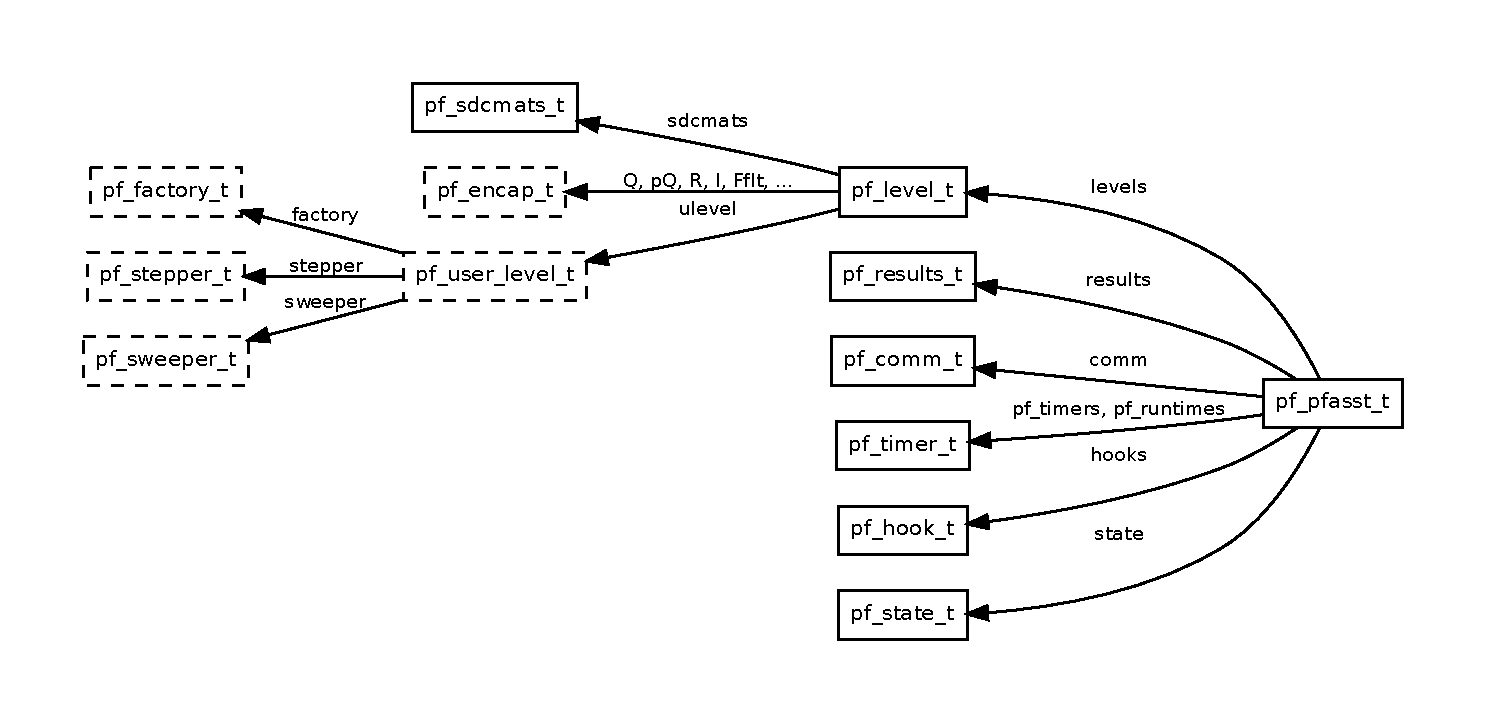
\includegraphics[width=\textwidth]{images/pf_pfasst_t.pdf}
  \caption{Hierarchy of derived types for LibPFASST's \protect\texttt{pf\_pfasst\_t}, generated using FORD\protect\footnotemark. Dashed outlines denote abstract types. An arrow from A to B indicates that type A contains one or more members of type B.}
  \label{fig:libpfasst_types}
\end{figure}
% END: ensure it's on the same page as the picture
\footnotetext{\url{https://github.com/Fortran-FOSS-Programmers/ford}}

In order to build and run LibPFASST, all members in this hierarchy must be referenceable (with the possible exception of \ilc{pf_stepper_t} and \ilc{pf_sweeper_t}, which may be omitted depending on LibPFASST parameters). For members of abstract types, this requires user code to explicitly initialize them using concrete child types before starting the run. Those can be broken down into two categories:
\begin{itemize}
    \item Abstract types with built-in concrete children: \ilc{pf_encap_t}, \ilc{pf_factory_t} and \ilc{pf_stepper_t}. For these, most use cases are covered by instantiating one of the built-in child types.
    \item Abstract types without built-in concrete children:
        \begin{itemize}
        \item \ilc{pf_user_level_t} has no built-in child types, so one must be defined by the user.
        \item \ilc{pf_sweeper_t} has multiple built-in child types, all abstract. Here the majority of use cases are better served by extending one of the child types, all of which are also abstract.
    \end{itemize}
\end{itemize}



\section{Extending Fortran derived data types in C} \label{sec:impl_oop}


\subsection{Type-bound procedures} \label{sec:impl_functions}

The reliance on abstract types by LibPFASST's design poses the main challenge driving the design of cpfasst, since there is no interoperability mechanism to allow the extension of a Fortran type in C. In fact, while both languages started out as strictly procedural, Fortran added object-oriented features over time, and with Fortran 2003 adding features to support inheritance and polymorphism, modern Fortran can be considered a full-fledged object-oriented language \cite{clerman2011modern}. Meanwhile, C remains strictly procedural, with the development of ``object-oriented C'' having branched off early on into a separate language, C++.

Having established the impossibility of implementing inheritance in the C code, we look into delegation. Delegation, when combined with composition, is a mechanism for code reuse as powerful as inheritance \cite{gamma1994design}. Strictly speaking, it is not possible to implement composition with delegation in C either: it relies on object orientation, and C has no concept of objects. However, it is possible to mimic its behavior well enough to leverage it for code reuse. More specifically, we choose to mimic an object-oriented design pattern that utilizes composition and delegation: the \textit{strategy} pattern.

The strategy pattern as shown in \cite{gamma1994design} allows encapsulation of different implementations of the a functionality, with the choice of which implementation to invoke happening at runtime. Its structure is illustrated here in \refFigure{fig:uml_strategy_pattern}. For our purposes, the "strategy" is the implementation-specific code to be provided by the user for a component of LibPFASST (e.g. sweeper, data encapsulation). One feature of this pattern makes it particularly well-suited for an interoperable interface: it can be used to avoid exposing data used by the strategy to the context \cite{gamma1994design}. This separation is critical for reliability, as we'll discuss in \refSection{sec:impl_data}.

\begin{figure}[ht]
  \centering
  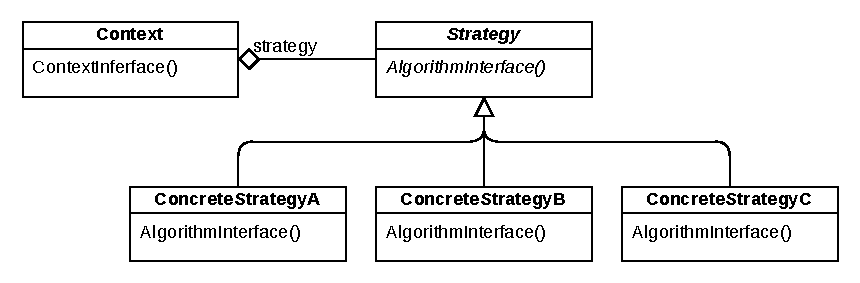
\includegraphics[width=\textwidth]{images/uml_strategy_pattern.pdf}
  \caption{UML class diagram showing the structure of the object-oriented strategy pattern, mimicked in the cpfasst implementation, as defined in \cite{gamma1994design}.}
  \label{fig:uml_strategy_pattern}
\end{figure}

A behavior akin to the object-oriented strategy pattern is implemented as follows, and illustrated in \refFigure{fig:uml_strategy_mimic}:
\begin{figure}[ht]
  \centering
  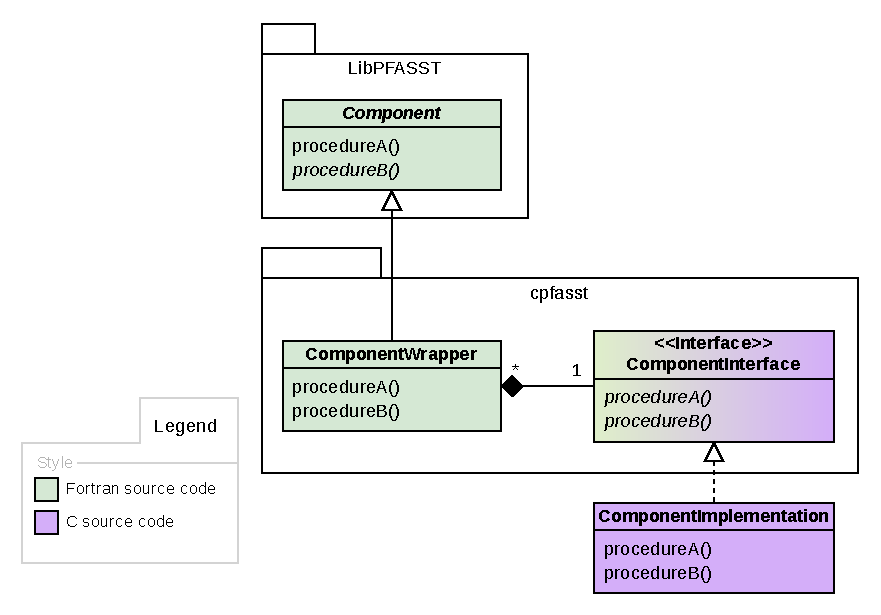
\includegraphics[width=\textwidth]{images/uml_wrapper_pattern.pdf}
  \caption{Pattern used to associate a LibPFASST component with a C implementation, in UML class diagram notation. The LibPFASST abstract component type is extended by a concrete wrapper, which forwards all calls to an interoperable interface, for which the user provides an implementation in C.}
  \label{fig:uml_strategy_mimic}
\end{figure}

\begin{itemize}
    \item For each of the LibPFASST abstract types involved, cpfasst defines, in Fortran, a concrete type extending it --- referred to from now on as a \textit{wrapper type}. The type defines the abstract methods from its parent, and can also override parent methods where needed. It wrapper acts as the pattern's \textit{context}, and all procedures it implements simply forward the call to the \textit{strategy}, performing data type transformations as needed.
    \item The Fortran cpfasst code also declares an interoperable procedure \textit{interface}, with external linkage, corresponding to each of the type's methods. A matching C header file provides equivalent function declarations. Together they act as the abstract \textit{strategy} class.
    \item The cpfasst user imports the header into a source file, and defines each of the contained methods. This implementation acts as the \textit{concrete strategy} class.
\end{itemize}

It's important to note that since the wrapper type delegates the call to specific C functions, this implementation differs from the pattern as used in object-oriented environments, as strategy selection happens at link-time, not runtime. This is a deliberate choice for performance reasons, which will be discussed in \refSection{sec:impl_restrictions}.

For a concrete example of how this pattern is applied, we examine the implementation of the cpfasst interface for the IMEX sweeper, illustrated in \refFigure
{fig:uml_imex_sweeper}. For simplicity, this section assumes the arguments and returns of all procedures to be interoperable, so that they can be passed in calls from Fortran to C without issue.

\begin{figure}[ht]
  \centering
  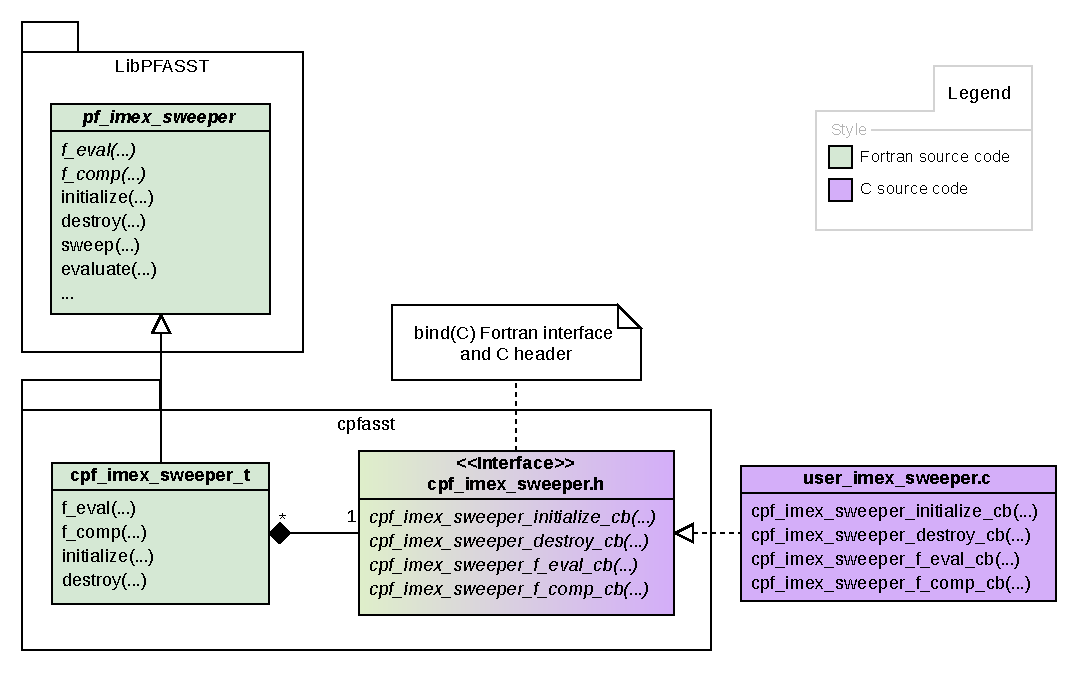
\includegraphics[width=\textwidth]{images/uml_imex_sweeper.pdf}
  \caption{cpfasst implementation of a wrapper type to LibPFASST's IMEX sweeper, in UML class diagram notation.}
  \label{fig:uml_imex_sweeper}
\end{figure}

As mentioned in \refSection{sec:libpfasst_usage}, use of this sweeper in Fortran consists of defining a type extending \ilc{pf_imex_sweeper_t}, and providing implementations
for its deferred type-bound procedures \ilc{f_eval} and \ilc{f_comp}. The cpfasst interface applies the previously described pattern to mimic this usage, implementing the
following elements:
\begin{itemize}
    \item The wrapper Fortran type, \ilc{cpf_imex_sweeper_t}. It provides implementations for \ilc{f_eval} and \ilc{f_comp}, forwarding calls to the corresponding C
    interfaces. Additionally, it also overrides two procedures from the parent type: \ilc{initialize} and \ilc{destroy}. The overriding implementations call both the parent procedure and the corresponding C callback, providing the C implementation an opportunity to initialize and destroy its own private data structures. Note that \ilc{pf_imex_sweeper_t} contains multiple other procedures which are not overridden: as there is no apparent reason why a cpfasst user would need to modify their behavior,
    adding a callback would only clutter the interface.
    \item The interoperable interface is declared twice: once in Fortran, through procedure interfaces with the \ilc{bind(C)} attribute, and once in the C header file 
    \ilc{cpf_imex_sweeper.h}. It is crucial for proper interoperability that the function signatures of both declarations are an exact match, and that types that
    convert between Fortran and C in non-trivial ways, such as character strings, are correctly handled.
\end{itemize}
The C user then imports \ilc{cpf_imex_sweeper.h}, and defines all the functions it declares. The \ilc{f_eval} and \ilc{f_comp} callbacks are an integral part of the solver
and must always be provided, but it is possible that the user implementation has no use for the \ilc{initialize} and \ilc{destroy} callbacks. However, because the
wrapper type calls these interfaces regardless, the C code must still define these functions, even if they are \textit{no-op}s.

\subsection{Data components} \label{sec:impl_data}

With the wrapper types providing referenceable members for all elements of the hierarchy from \refFigure{fig:libpfasst_types}, it is possible to build and run an executable that invokes the C functions at the appropriate contexts. Those functions would be limited to operating on their argument lists, but maintaining the assumption from \refSection{sec:impl_functions} that the argument and return types of all involved procedures are interoperable, this would be sufficient for a simple use case. In fact, LibPFASST's first tutorial, a solution of the 1D Dahlquist test equation, could be replicated in this scenario.

Implementing non-trivial problem-specific behavior under those restrictions, however, is a different matter. When defining a type-bound procedure for one of the extended LibPFASST types in Fortran, the user has full access to the data components from their derived type, and those inherited from the parent type. It follows that cpfasst must provide a mechanism for the C user to achieve similar functionality.

For this, we look again to the object-oriented strategy pattern. As previously mentioned, it provides separation of data between context and strategy --- each of the classes have access to their own member variables, and data is shared between them only through function arguments. When converting from inheritance in a situation where child classes commonly access members variables of the parent class, this can lead to extensive argument lists. Fortunately, this is not the case with LibPFASST. While its code makes little use of accessibility statements for derived type components, and Fortran defaults to public access, its abstract classes are self-contained, with little need for child types to access to parent data --- in fact, it can be argued that LibPFASST components such as the sweeper and user level would be better served by using delegation than inheritance for problem-specific behavior, even Fortran-only code. Where access to parent data is needed, it is restricted to program initialization, by setting parent class variables that control execution behavior. Hence, the same functionality can be covered either by setting those variables during initialization using values provided by a C callback, or by providing get/set interoperable interfaces in Fortran that the C code can call as needed. 

Member data of the strategy class is part the cpfasst user's C code, and as such can be implemented as they see fit --- within some restrictions, which will be discussed in \refSection{sec:impl_restrictions}. It would possible, in fact, to leverage a different object-oriented language's interoperability with C, and implement them as actual members of an object in that language. For C code, the examples provided in with cpfasst illustrate some strategies for implementing data with the desired behavior: for instance, data shared across all objects of a class (equivalent to a C++ static data member) can be represented by a C global variable, in a scope visible to all functions composing the ``class''. This is often the case with problem parameters, such as physical constants or dimensions.

However, there is no easy representation in a purely procedural language for a regular data member (unique to each object). As mentioned in \refSection{sec:impl_functions}, cpfasst is restricted to a single strategy --- a single C ``object'', emulating the functionality of multiple Fortran objects of the same class in LibPFASST. A popular way to emulate this behavior in C --- and, in fact, the way many object-oriented languages, such as C++ and Python, implement class method calls --- is to pass as the first function argument a reference to the ``object'' (a C \ilc{struct} containing the data members). Since in our case the function call comes from Fortran, the Fortran wrapper type must store the reference and pass it as needed: it does so through the interoperable opaque derived type \ilc{c_ptr}. 

\begin{figure}[ht]
  \centering
  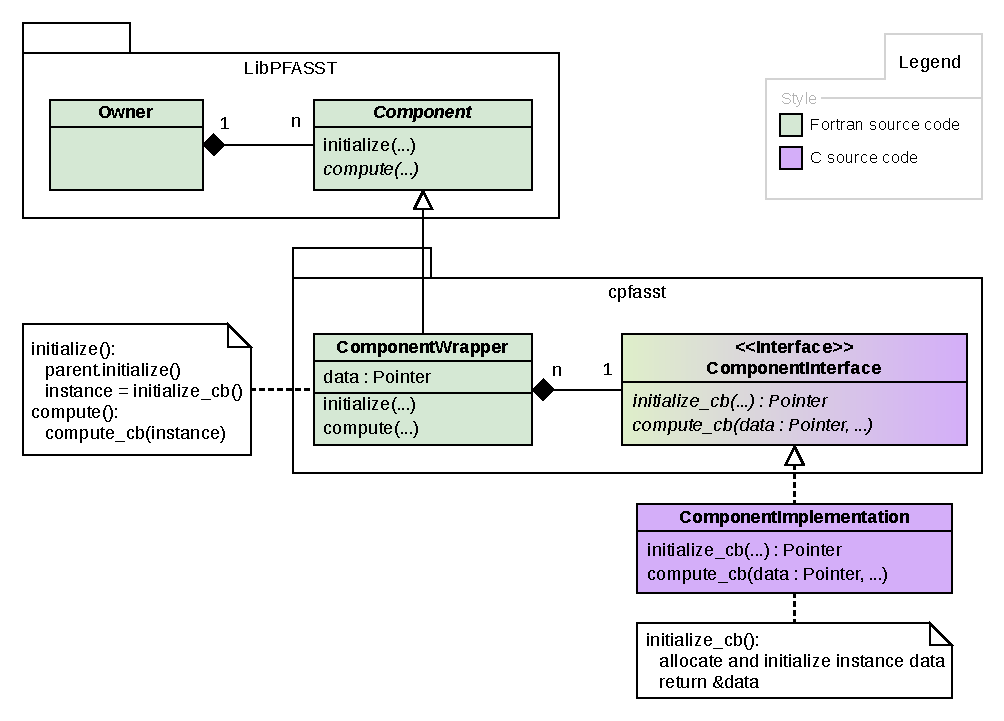
\includegraphics[width=\textwidth]{images/uml_strategy_data.pdf}
  \caption{Pattern used to emulate the behavior of object-oriented data members by the cpfasst interface, in UML class diagram notation. The wrapper type stores a C pointer, which is included as an argument in calls to C callback functions. The data referenced by this pointer is owned by the user's C code, and opaque to the Fortran implementation.}
  \label{fig:uml_strategy_data}
\end{figure}

\refFigure{fig:uml_strategy_data} revisits the diagram from \refFigure{fig:uml_strategy_mimic}, with an emphasis on data members and multiplicities. While the pointer to the user data is stored by the Fortran wrapper type, the data itself is owned by the C code. This includes, if applicable, responsibility for allocating dynamic memory on initialization, and deallocating it on destruction (a callback function not shown in the figure). The wrapper type never changes the pointer's value, and in most cases does not dereference the pointer at all --- the one exception being the wrapper for LibPFASST's data encapsulation type, as detailed in \refSection{sec:impl_functions}.


\subsection{Forwarding non-interoperable procedure calls} \label{sec:impl_calls}

With an understanding of the mechanics cpfasst utilizes for extending Fortran types, we can understand its exact scope. Wrapper types are provided for the abstract types shown in \refFigure{fig:libpfasst_types}: \ilc{pf_encap_t}, \ilc{pf_factory_t} and \ilc{pf_user_level_t} are wrapped directly, but for \ilc{pf_sweeper_t}, only abstract child type \ilc{pf_imex_sweeper_t} is wrapped: interoperable interfaces for other sweepers are outside the scope. Also left outside the scope is \ilc{pf_stepper_t}: it represents a sequential time stepper, and is used only when specified by LibPFASST configuration, for execution of Parareal or for initialization of the coarse level in PFASST --- the respective configuration values are, consequently, not supported. The wrapper functions have the same name as their parents, with the prefix \ilc{pf} replaced by \ilc{cpf}.

In \refSection{sec:impl_oop}, all arguments of type-bound procedures in the wrapper type were assumed to be either of an interoperable type, or easily converted into one. That assumption only holds for a small minority of the procedures the wrapper types must define: most of these procedures take arguments of other derived types. This means we must evaluate interoperability not only for our wrapper types, but also for the types of all arguments in procedures they define (procedures for which a parent definition is inherited are not relevant, as they are not part of the C interface). The results of this analysis are shown in \refFigure{fig:libpfasst_dependencies}.

\begin{figure}[ht]
  \centering
  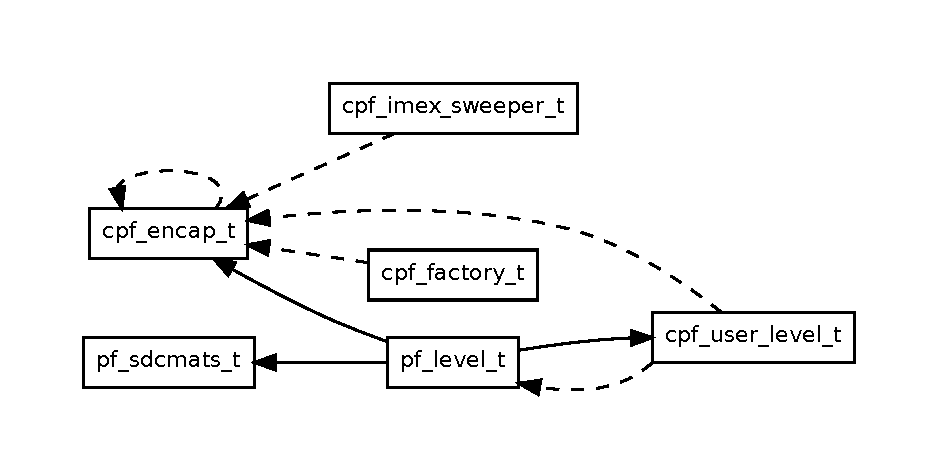
\includegraphics[width=\textwidth]{images/pfasst_dependencies.pdf}
  \caption{Type dependencies of procedures defined by cpfasst wrapper types. A dashed line from A to B indicates that type A contains one or more members of type B. A continuous line from A to B indicates that cpfasst wrapper type A defines a procedure containing an argument of type B (ignoring references to the owner instance).}
  \label{fig:libpfasst_dependencies}
\end{figure}

First, we focus on LibPFASST types appearing in the dependencies: \ilc{pf_level_t} and \ilc{pf_sdcmats_t}. \ilc{pf_stepper_t}, as previously mentioned, is not used within the scope of cpfasst, and can be ignored. Ideally, the remaining types would be interoperable, so that they could be forwarded to the C interfaces without issue: they are not, and cannot easily be converted as they all contain allocatable types. A significant amount of time was spent during development investigating different approaches for interfacing with non-interoperable Fortran types, and the viable strategies created are presented in Appendix \ref{sec:derived_type_interface}. It was ultimately concluded that any maintainable implementation of such an interface for LibPFASST would involve the development of a code generator, and even then might fail to provide the necessary performance for use in the wrapper classes, as all involved procedures are part of the main PFASST execution loop. 

At this point, we approached the issue from a new perspective: how can the non-interoperable types be eliminated from the C interface with minimal restrictions being placed on the cpfasst user? For this, we evaluate each type under the criteria: is there a clear use case where the user needs access to this type? If so, to which components?

\ilc{pf_level_t} appears as an argument in the interpolation and restriction operations, but is not required as an input or output to them: instead, its intended purpose seems to be providing access to the full context of the levels involved. In LibPFASST tutorial and test code, \ilc{pf_level_t} is only used in this context to access user-defined sweeper components for the same level --- this is something the C user's code can easily implement, if needed, based only on that level's index. This allows arguments of \ilc{pf_level_t} to be replaced in the C interface by their respective level indices. Note that access to other members of \ilc{pf_level_t} through the C interface is needed in different contexts, which will be covered separately. \ilc{pf_sdcmats_t}

Having eliminated the dependencies on LibPFASST types, we evaluate the dependencies on the cpfasst wrapper types themselves. While major components of the interoperable interface, they are themselves not interoperable, as they extend other types. This is a considerably easier analysis: a single wrapper type is depended on by all others (including itself), \ilc{cpf_encap_t}. 

\ilc{pf_encap_t} is what is known in other object-oriented languages as a \textit{pure abstract} or \textit{interface} class: it has no data components, and all its type-bound procedures are deferred. As such, when implementing the wrapper \ilc{cpf_encap_t}, there is no need to worry about whether any parent members must be accessible to its procedures, or whether any parent procedures must be overridden to enable extension in C code. Additionally, since the parent has no data components, and according to the mechanisms shown in \refSection{sec:impl_data}, any data components owned by \ilc{cpf_encap_t} are defined in the cpfasst user's C code. Therefore, a dummy argument of type \ilc{cpf_encap_t} can be replaced in the interface by its data pointer.

\section{Initializing LibPFASST components in C} \label{sec:impl_initializing}

In \refSection{sec:impl_oop} we examined how cpfasst allows the user to provide an implementation in C for functionality of LibPFASST types. At this point, it would be possible to run cpfasst code where the solution in space is implemented in C, and LibPFASST initialization and configuration are implemented in Fortran. This might be sufficient for a user comfortable with both languages, but the goal for cpfasst, as mentioned in \refSection{sec:impl_design_goals}, is to support user implementation entirely from C code, hence, we must provide interfaces for initialization and configuration as well. This is approached with a different mindset from the wrapper interfaces: there is no concern for performance, as these steps account for a minimal fraction of the time spent in execution for a real-world application of LibPFASST. Instead, focus is fully shifted into making the interface intuitive and maintainable.

Initialization and configuration in Fortran code involves calls to a few different LibPFASST procedures, as well as allocation and initialization of Fortran user types. Here we run into the same issue described in \refSection{sec:impl_calls}, as the LibPFASST procedures called involve non-interoperable derived types, but in a much more forgiving context. Proper implementation of wrapper types as defined in this work requires that each type-bound procedure call to be forwarded to an equivalent C function, but the procedural nature of initialization and configuration imposes no such constraints: as long as all Fortran steps are executed in a reasonable order, the manner in which they are presented to the C user is of no consequence to LibPFASST operation. In this section, we split this process into three major sections, and examine how each was adapted for the C interface.

\subsection{PFASST configuration} \label{sec:impl_pfasst_config}

This step boils down into correct initialization of the LibPFASST \ilc{pf_pfasst_t} type, which contains variables controlling all LibPFASST configurations, as well as all LibPFASST work variables. In Fortran code, it follows the following sequence:

\begin{enumerate}
    \item \label{config_step_mpi} Initialize MPI by calling \ilc{MPI_Init} \label{config_step_init}
    \item \label{config_step_comm} Initialize the LibPFASST communicator \ilc{pf_comm_t} by calling \ilc{pf_mpi_create} with the appropriate MPI communicator handle
    \item \label{config_step_prm} Initialize the main LibPFASST type \ilc{pf_pfasst_t} by calling \ilc{pf_pfasst_create}, providing the previously initialized \ilc{pf_comm_t}. Optional arguments control how LibPFASST parameters are initialized, which the user can mix as desired. If a value is not provided for a parameter, it is set to a working default (except for \ilc{nlevels}, the number of desired PFASST levels, which is mandatory).
    \begin{itemize}
        \item \ilc{nlevels} can be used to provide a value directly for the mandatory parameter;
        \item \ilc{fname} can be used to provide a path to a file in the Fortran Namelist I/O (nml) format, and the values contained will override LibPFASST defaults;
        \item Unless \ilc{nocmd} provided and set to true, parameters provided in the command line are also read, overriding defaults and those provided by other means.
    \end{itemize}   
\end{enumerate}

Two derived types are involved: \ilc{pf_comm_t} is an internal component of LibPFASST with no contents of interest to the user, so there is no reason to expose it in the C interface. \ilc{pf_pfasst_t}, on the other hand, houses both a set of internal work variables of no interest, and the LibPFASST parameters, which are the key component in this section and must be exposed to the C user. While the internal work variables are non-interoperable, all the parameters are of intrinsic Fortran types, and could easily be converted into interoperable types: taking this into consideration, we evaluated splitting this type into two, with one of the resulting derived types containing only parameters and being interoperable. However, it is unlikely that such a change would be accepted into LibPFASST purely for setup convenience. Even assuming the change was accepted, allowing the interoperable structure containing the parameters to be shadowed in the C interface and directly manipulated by the cpfasst user, the resulting interface might still be unintuitive for use in C code, as it would require character strings to be set according to Fortran convention.

Taking this into consideration, both \ilc{pf_pfasst_t} and \ilc{pf_comm_t} are excluded from the C interface. Step \ref{config_step_mpi} is left to the user's code, allowing MPI to be initialized through the C interface with the desired parameters. Steps \ref{config_step_comm} and \ref{config_step_prm} are condensed in a single interoperable subroutine, \ilc{cpf_initialize}, which takes as arguments the communicator handle obtained from the MPI C interface, and the arguments \ilc{nlevels} and \ilc{fname} from step \ref{config_step_prm}. This subroutine handles the conversion of the MPI handle from C to Fortran (using \ilc{MPI_Comm_f2c}), and the conversion of \ilc{fname} from C string to Fortran string. Argument \ilc{nocmd} is not exposed by the interface, and always set to true in the call to \ilc{pf_pfasst_create} --- testing reveals that the Fortran command line tools are incompatible with a \ilc{main} routine implemented in C, so this feature of LibPFASST cannot be supported.

After the \ilc{cpf_initialize} call, the user can retrieve the resulting parameter values by instantiating the interoperable type \ilc{cpf_parameter_struct}, and initializing it through interoperable subroutine \ilc{cpf_get_parameters}. This copies the relevant parameter values from \ilc{pf_pfasst_t} into a separate interoperable \ilc{struct}, handling string conversions. A corresponding subroutine \ilc{cpf_set_parameters} can be called to copy the values back into \ilc{pf_pfasst_t}, handling string conversions and validating parameter values against any cpfasst restrictions in the process. This is the intended way to initialize parameters for cpfasst, with the nml initialization option being included only as an easy path to reproduce LibPFASST configurations from Fortran for testing.

\subsection{Level configuration}

This step consists of manually instantiating problem-specific components on each of the PFASST levels, as mentioned in \refSection{sec:libpfasst_arch}. The Fortran implementation steps are, for each of the levels:
\begin{enumerate}
    \item Allocate \ilc{pf_user_level_t} using the user-provided concrete type.
    \item Allocate the applicable components of \ilc{pf_user_level_t}: \ilc{pf_factory_t}, \ilc{pf_sweeper_t}, \ilc{pf_stepper_t} using user-provided concrete types or built-in types (where applicable).
    \item \label{config_step_bufsize} Call LibPFASST subroutine \ilc{pf_level_set_size}, providing information about the shape of numeric data used to store the solution for this level.
\end{enumerate}

For cpfasst, the first two steps are straightforward: the wrapper types for each of the LibPFASST types are used, and, as explained in \refSection{sec:impl_calls}, \ilc{pf_stepper_t} is ignored. Step \ref{config_step_bufsize}, however, requires user input: when initializing from Fortran code, the provided shape is used to calculate the size for the MPI buffer used to communicate the level's solution between processors, and on calls to \ilc{pf_factory_t}, where it specifies the desired shape for the data. The latter is only relevant for the built-in factory types (in fact, to avoid confusion regarding row-major/column-major, the corresponding argument is omitted from the C callbacks for \ilc{cpf_factory_t}), but the former is fundamental for correct communication when running with more than one processor.

The \ilc{pf_level_set_size} subroutine takes an optional argument, \ilc{buflen_in}, which allows for directly setting the buffer to the desired length. This is not the storage size, but the required length of a buffer of type \ilc{real(pfdp)} to provide sufficient storage for the solution data. Since the cpfasst solution data is specified in C code by the user and opaque to the Fortran implementation, information about its storage size on each level must be provided by the user in order to correctly configure the MPI buffer.

As before, the steps are condensed into a single interoperable subroutine, \ilc{cpf_initialize_level}, which takes as arguments the level index (zero-based, in accordance with C convention) and the storage size of the solution in bytes. It then allocates all the required wrapper types, converts the solution size to the equivalent buffer length (rounding up if needed) and calls the \ilc{pf_level_set_size}, with a dummy shape of \ilc{[1]} and the calculated buffer length.

\subsection{Running PFASST}

At any point before starting the run, the user must call two cpfasst interoperable subroutines:
\begin{itemize}
    \item \ilc{cpf_set_initial_condition} accepts a reference to an instance of the user-defined solution type, at the finest spatial discretization level,  initialized to the desired initial condition;
    \item \ilc{cpf_set_solution_storage} accepts a separate reference to an instance of the user-defined solution type, at the finest spatial discretization level, which will be used by cpfasst to store the final result of the run.
\end{itemize}
The user retains ownership of this memory, and is responsible for freeing it if dynamically allocated, but must not do so until the run has concluded. The remaining Fortran code steps to start the run are:
\begin{enumerate}
    \item Call LibPFASST subroutine \ilc{pf_pfasst_setup}, which performs final setup steps on the \ilc{pf_pfasst_t}
    \item Call LibPFASST subroutine \ilc{pf_pfasst_run}, providing the desired time step size for the solution, as well as the total number of time steps, which must be a multiple of the number of processors used. This starts PFASST execution.
\end{enumerate}

cpfasst interoperable subroutine \ilc{cpf_run} takes the two arguments described in the second step. It checks that the initial and final condition pointers have been set, then executes the two steps above, starting the run, and returns only when the run is complete. At this point, the user can read the solution from the provided memory. Memory allocated by the Fortran code, or by the user as part of the \ilc{cpf_factory_t} callbacks, should be freed by calling cpfasst subroutine \ilc{cpf_pfasst_destroy}, which calls the LibPFASST procedure of the same name, prompting LibPFASST to free all memory it allocated --- including invoking the \ilc{cpf_factory_t} callbacks to free allocated memory tied to the data encapsulation pointers.


\section{Restrictions of cpfasst functionality} \label{sec:impl_restrictions}

As discussed in \refSection{sec:impl_design_goals}, one of the driving purposes in the development of cpfasst was to expose through the C interface as much of the functionality provided to the Fortran LibPFASST user as possible. However, as mentioned in previous sections, some compromises were imposed by limitations of interoperability, and others by compromises with other design goals. In this section, we detail these limitations and the reasons behind them.

\subsection*{Static linking of callback functions}

As mentioned in Section \refSection{sec:impl_functions}, the cpfasst wrapper types are linked through binding labels to specific C functions. Association of different implementations of user types with different levels can be desirable for purposes such as the use of reduced physics at a coarser level, and is easily achievable for the Fortran user through the creation of different types extending the same LibPFASST abstract type, which are then instanced at the appropriate level. It is possible to implement a wrapper type that behaves in the same manner, by using \ilc{bind(C)} procedures with no binding labels for the callbacks, and the interoperable C function pointer type: the wrapper instance would store C function pointers to each of its callbacks, which would be initialized by the cpfasst user during configuration steps. Aside from the more flexible functionality, the resulting cpfasst interface would arguably be made more intuitive by having the user purposefully provide function pointers to the callbacks, rather than being required to provide definitions for them with specific names.

However, the callback functions are invoked countless times during PFASST execution, and as such, in order to minimize the performance overhead of cpfasst, it is desirable that link-time optimization should be able to apply interprocedural optimizations between the two languages. The GCC 10.1.0 documentation explicitly mentions this feature, but it appears to be limited to direct calls, as testing revealed that functions called through pointers are never inlined. Additionally, link-time warnings about type size mismatches, which are extremely useful for detection of issues in the interoperable interfaces, are not generated for a call made through a function pointer. For this reason, this concept was abandoned in favor of the one presented in this work.

\subsection*{Limited wrapper type callbacks}

When extending abstract types containing non-deferred type-bound procedures, the Fortran user of LibPFASST has the freedom to choose which parent procedures to override, based on problem-specific needs. Due to the static linking of the callback interfaces, however, cpfasst cannot extend this flexibility to the C user: if a wrapper type overrides a parent procedure, forwarding the call to a C callback interface, its definition must be provided by the user in C code. If it does not, the C code has no way to modify that procedure. For some procedures, such as \ilc{initialize} and \ilc{destroy} from \ilc{pf_sweeper_t}, there is a clear use case for overriding them, equivalent to constructor and destructor overriding in other object-oriented languages: just as in those languages, the wrapper type first calls the parent initialization method, then the C callback (corresponding to the child's constructor), with destruction being done in the opposite order. For other procedures, however, even if a callback were provided, should it be invoked before or after the parent procedure? Or replace it entirely? Since there is no clear use case, the inclusion a callback for each parent procedure serves only to increase the complexity of the interface. Thus, we provide callbacks only for deferred type-bound procedures of the parent types, as well as initialize and destroy methods.

\section{Verifying the interoperable interface} \label{sec:impl_verification}

Verification is made significantly harder in multi-language environments. Static code analysis tools and compiler checks are limited to a single language, so while code in each language can be thoroughly checked, the interaction between them remains a potential source of issues. Runtime checks based on code generation in one of the languages are also affected by this, like the checks enabled by gfortran's \ilc{-fcheck=<keyword>} flag. In this section, we highlight tools found during this work to facilitate detection of issues arising from the interaction between languages.

Here it is assumed that all interfaces involved make use of Fortran 2003 C bindings, which, as detailed in \refSection{sec:interop_f03}, preclude multiple issues arising from differences in the low-level representation of a procedure between C and Fortran. Under this assumption, the single major sources of bugs identified is the presence of mismatched representations of an interoperable entity between the two languages.

As explained in \refSection{chapter:interoperability}, every interoperable procedure and type requires a matching representation in Fortran and C. When those representations do not match, it is likely that the code will not operate properly. Unit testing is sufficient to identify more straightforward issues, but others can be extremely hard to diagnose: in the development of cpfasst, a mismatch in the length of a string caused Fortran to read past the bounds of the type it was contained in. This manifested as a segmentation fault, not where the out-of-bounds access occurred, but wherever the next memory allocation was attempted afterwards, and only when running problems above a certain size --- the issue was identified and fixed using the tools discussed here, but the exact reason for how it manifested remains unknown. In \refSection{sec:interop_f90_strings} we discussed a similarly hard to diagnose issue which affected multiple scientific computing tools relying on Fortran 90 interoperability in 2019, the root cause of which was found to be an interface mismatch that had been present for years. It follows that ensuring matching between representations is a critical part of verifying the interface.

\subsection*{Automatically generated headers}

It is possible to automatically generate C headers matching the Fortran representation of interoperable entities using the GNU Fortran compiler's \ilc{-fc-prototypes} flag. In cpfasst, the generated headers were deemed unsuitable for use as the ``official'' interface headers, as prototypes from included modules get placed in a single file, arguments are unnamed, and comments are not carried over. Instead, it was proposed that the generated headers should be included not instead of, but in addition to the manually written ones ---  if the different declarations are not compatible, the compiler stops with a conflicting types error. The downside of using this method is that the error cannot be downgraded into a warning, and sometimes a mismatch in pointer types is deliberate, since the manually written interface includes context that the automatically generated one lacks.

Consider a scenario (for instance, the one described in \refSection{sec:impl_calls}) where the C code passes a pointer to data of arbitrary non-interoperable type to a Fortran procedure, which is then forwarded to a call to a C function: the type of the argument in the Fortran interface declaration is \ilc{type(c_ptr)}, which it translates into the C header as \ilc{void*}. The implementation, however, requires that the referenced data be of a certain type on the first call, and guarantees that it will be of that type on the second --- it makes sense that the pointer type on the manually written header should reflect that. However, when using the generated headers as described above, the mismatch in the pointer type will cause a compilation error, so this trade-off must be considered. The same issue occurs with \ilc{type(c_funptr)}, which generates a pointer of format \ilc{int(*)()}.

\subsection*{Link-time type checks}

One of the best tools for verification of the interoperable interface is easily overlooked, as it is not usually considered a verification tool at all: enabling link-time optimization. When this feature is enabled, the compiler saves its intermediate representation to disk, allowing a single optimization pass at link-time that is not limited to the context of each compiling unit. In GCC, the additional information is also used to perform correctness checks in the types of function arguments: this applies to intrinsic and derived types, passed by reference or value. An example is shown in \refSrc{src:lto_warnings}. In a single-language environment, these additional checks are superfluous, as type mismatches will generate warnings or errors at compile-time. Where the interoperable interface is concerned, however, they are great asset in identifying mismatches between the declaration of the same interface in both languages. Hence, it is strongly recommended that even if link-time optimization is not desirable in a project, it should still be employed for validation.

\begin{listing}
    \inputminted{Fortran}{src/misc/lto_warnings/fsrc.f90}
    \inputminted{C}{src/misc/lto_warnings/csrc.c}
    \inputminted[fontsize=\small]{text}{src/misc/lto_warnings/output.txt}
    \caption{Mismatched declarations of the procedure in C and Fortran cause the code to print incorrect values, but no warnings are generated when linking normally with GCC v10.1.0. With link-time optimization enabled (\ilc{-flto}), type mismatch warnings are issued for both function calls, only one of which is shown here.}
    \label{src:lto_warnings}
\end{listing} 

Since it emits warnings instead of errors, the use of link-time optimization allows the developer to evaluate whether a mismatch is cause for concern and ignore the warning if not. Its main drawbacks are increased compiling and linking time and increased size of the intermediate binaries. Additionally, as mentioned in \refSection{sec:impl_restrictions}, function pointers were found through testing to obfuscate the context of a call to GCC link-time optimization, so calls made through a function pointer are not subject to these checks.

\subsection*{Memory access checks}

Validation of the interface through either of the above methods was found sufficient to ensure equivalence of interoperable entity representations, in the context of the interfaces used for this project. But having correct interface declarations is, as in single-language programs, not sufficient to avoid out-of-bounds memory access in the code using it. Those issues can either arise from the wrapper function code, or from the user's code. The wrapper code is part of the interface, and hence part of the verification process: while Fortran is less prone to out-of-bounds access issues than C, interoperable interfaces often rely on some Fortran intrinsic functions that undermine this robustness by doing the equivalent of a C \textit{cast}, such as \ilc{transfer}, \ilc{c_f_pointer} and \ilc{c_f_procpointer}. Additionally, as previously mentioned, the header generation and link-time check methods are flawed where interoperable Fortran types \ilc{type(c_ptr)} and \ilc{type(c_funptr)} are involved, necessitating the use of additional validation methods to cover those sections.

When it comes to issues in user code, they are not within the scope of interface verification. Nevertheless, it is advisable to offer the user information about verifying their code specifically in the context of interoperable use, as the C/Fortran application seems to be far more sensitive to incorrect memory access than C applications, which are largely unaffected by out-of-bounds reads in memory owned by the program. Furthermore, as mentioned earlier in this section, these issues may not manifest in the manner the C user expects --- of the memory access issues found during development of cpfasst, only a small minority manifested as a segmentation fault tracing back to the instruction where the access occurred --- making information about which tools to use all the more helpful.

Valgrind Memcheck\footnote{\url{https://www.valgrind.org/}} is a well-known tool for dynamic analysis of memory access with MPI support. It instruments a number of instructions related to memory access, detecting accesses to unaddressable memory, memory leaks at program termination, memory aliasing in arguments to functions such as \ilc{strcpy} and \ilc{memcpy}, and use of undefined memory \cite{seward2005using}. Equally relevant in this context is what it does not detect: an access is only considered out-of-bounds by Valgrind when it happens past the boundary of an allocated block on the heap, or on at an invalid address on the stack. An access out-of-bounds in the stack or global memory, for instance, will go undetected so long as it happens in memory the program can legally access. Use of the tool remains recommended, as it would be in a single-language environment, but it was found insufficient for detection of potentially fatal issues in for mixed-language program, and hence should not be solely relied on in such a scenario.

AddressSanitizer\footnote{\url{https://github.com/google/sanitizers/wiki/AddressSanitizer}} is a memory error detector tool, consisting of a compiler instrumentation module and a run-time library. It has been included with GCC since version 4.8, through the \ilc{-fsanitize=address} compiler flag. Its functionality partially overlaps with Valgrind's, but because unlike Valgrind it is able to detect out-of-bounds accesses not only in the heap, but also in the stack and in global memory, as exemplified in \refSrc{src:asan}. It does so by surrounding each variable with ``poisoned'' memory segments, and detecting any access to those segments, both in Fortran and C code. Its main drawback is the need to recompile the code for instrumentation, but at an average memory overhead of 3.4x and runtime increase of 1.73x \cite{serebryany2012addresssanitizer}, it is lightweight enough to be used in development builds for most applications. It is strongly recommended that AddressSanitizer or an equivalent tool be used during verification of interoperable interfaces and user code relying on them.

\begin{listing}
    \inputminted{Fortran}{src/misc/asan/fsrc.f90}
    \inputminted{C}{src/misc/asan/csrc.c}
    \inputminted[fontsize=\small]{text}{src/misc/asan/output.txt}
    \caption{Interoperable code with out-of-bounds memory access in global memory due to mismatched array lengths, and corresponding AddressSanitizer output (edited for brevity). Out-of-bounds accesses in the stack and global variables are not detected by Valgrind Memcheck.}
    \label{src:asan}
\end{listing} 